\chapter{Использование инструментов анализа производительности запросов}
\section{Основные понятия оптимизации запросов}
\subsection{Проблемы оптимизации запросов и оптимизатор запросов}

SQL Server может выполнять объединение разными способами. Он может использовать любой из следующих алгоритмов объединения: 

\begin{itemize}
	\item вложенные циклы (Nested Loops); 
	\item слияние (Merge); 
	\item хэш (Hash); 
	\item хэш оптимизированной фильтрации по битовым картам (Bitmap Filtering
	Optimized Hash, также называемый оптимизацией типа "звезда"). 
\end{itemize}


Прежде чем продолжить рассматривать процесс оптимизации запросов, в данном
занятии мы кратко опишем, как SQL Server выполняет запросы. 

\begin{figure}[h!]
	\begin{center}
		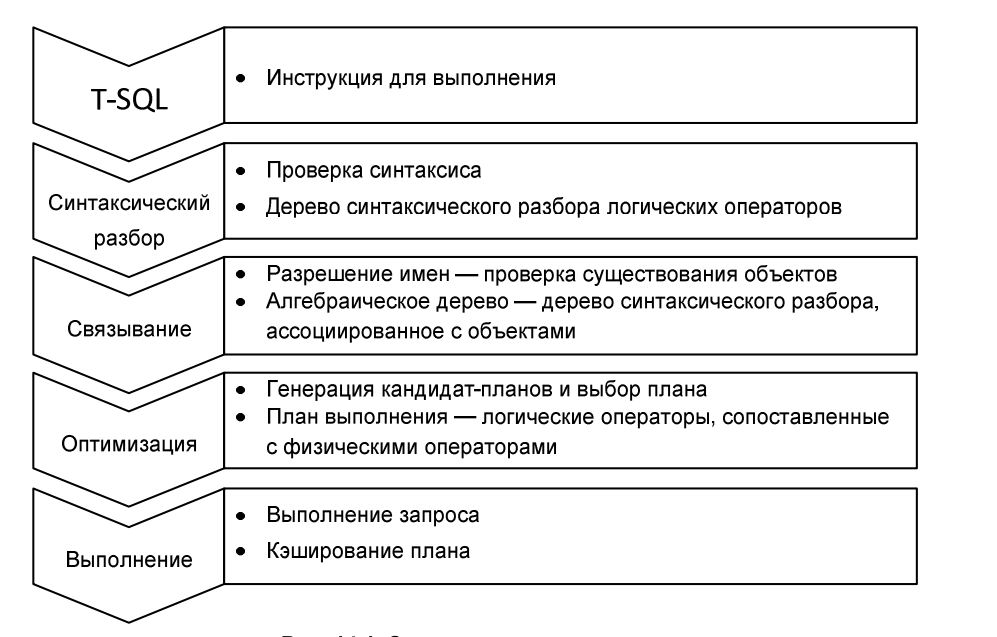
\includegraphics[width=0.9\textwidth]{img/stages2.png}
	\end{center}
	\captionsetup{justification=centering}
\end{figure}

Сниффинг параметров — это процесс, когда SQL Server пытается перехватить
(sniff) значение текущего параметра в процессе компиляции и передает его оптимизатору запросов.

SQL Server проделывает огромную работу по оптимизации запросов и поддерживает
кэшированные планы. Но существует множество ситуаций, когда что-то идет не так,
как нужно, и выбирается не лучший план, как, например, в следующих сценариях:

\begin{itemize}
	\item выбран не лучший план, поскольку область поиска планов выполнения была
	слишком большой; 
	\item статистическая информация не представлена или не обновлена, что ведет к неправильной оценке мощности; 
	\item кэшированный план является неоптимальным для данного значения параметра; 
	\item перехват параметров ведет к неточной оценке мощности; 
	\item оптимизатор запросов недооценивает или переоценивает стоимость алгоритма,
	реализованного в физическом операторе;
	\item изменения в аппаратном обеспечении могут больше соответствовать другому
	плану выполнения. Например, кто-то мог добавить в блок процессоры, и план,
	который использует большее время центрального процессора (ЦП), может быть
	более подходящим. 
\end{itemize}

\begin{figure}[h!]
	\begin{center}
		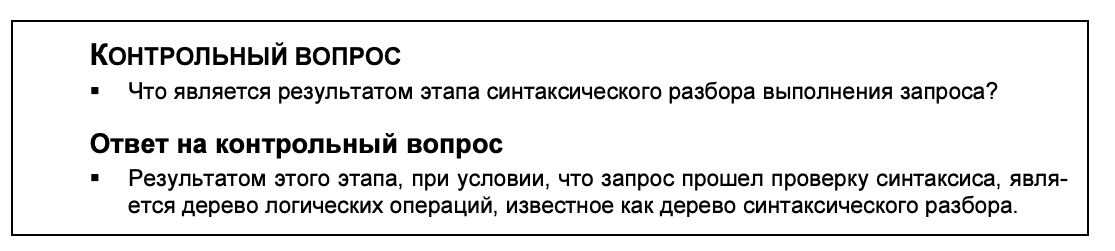
\includegraphics[width=0.9\textwidth]{img/zakrep33.png}
	\end{center}
	\captionsetup{justification=centering}
\end{figure}



\subsection{Подсистема расширенных событий SQL Server, трассировка SQL и приложение SQL Server Profiler}

Пакет расширенных событий представляет собой контейнер всех объектов подсистемы расширенных событий. К этим объектам относятся следующие. 

\begin{itemize}
	\item \textbf{События (Events)}. Это точки мониторинга, которые вас интересуют. Можно
	использовать события для мониторинга или для запуска синхронных или асинхронных действий. 
	\item \textbf{Цели (Targets)}. Это получатели событий. Можно использовать цели, которые
	выполняют запись в файл, хранят данные события в буфере памяти или собирают статистические данные о событиях. Цели могут выполнять синхронную или
	асинхронную обработку данных.
	\item \textbf{Действия (Actions)}. Это ответы на события. Они привязаны к событию. Действия могут получать копию стека и проверять данные, сохранять информацию в
	локальной переменной, собирать статистические данные о событиях и даже добавлять данные к данным события. Например, в SQL Server можно использовать
	действие обнаружения плана выполнения для нахождения плана выполнения. 
	\item \textbf{Предикаты (Predicates)}. Это наборы логических правил для фильтрации собранных событий. Для минимизации влияния сессии мониторинга на систему
	важно захватывать только нужные события. 
	\item \textbf{Типы (Types)}. Они помогают интерпретировать собранные данные. В действительности, данные — это коллекция байтов, а типы представляют контекст данных. Тип имеют события, действия, цели, предикаты и сами типы. 
	\item \textbf{Карты (Maps)}. Это внутренние таблицы SQL Server, которые отображают внутренние числовые значения на значимые строки. 
\end{itemize}

Трассировка SQL (SQL Trace) — это встроенный механизм для получения
событий. 

\begin{figure}[h!]
	\begin{center}
		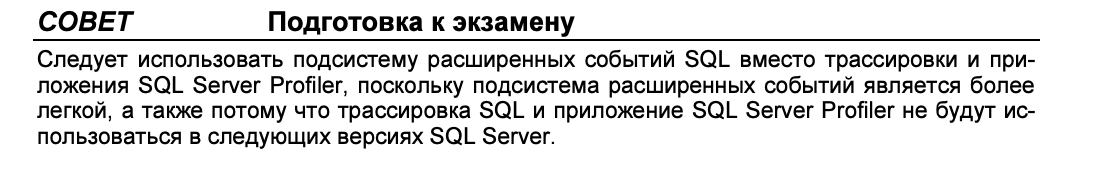
\includegraphics[width=0.9\textwidth]{img/advice40.png}
	\end{center}
	\captionsetup{justification=centering}
\end{figure}


\subsection*{Резюме занятия}
\begin{itemize}
	\item Оптимизатор запросов генерирует кандидат-планы выполнения и оценивает их. 
	\item SQL Server предоставляет множество инструментов, которые помогают пользователям анализировать запросы, включая подсистему расширенных событий,
	трассировку SQL и приложение SQL Server Profiler. 
	\item Подсистема расширенных событий является более легким механизмом мониторинга, чем трассировка SQL. 
	\item SQL Server Profiler предоставляет пользовательский графический интерфейс для
	доступа к трассировке SQL. 
\end{itemize}

\subsection*{Закрепление материала}

\begin{figure}[h!]
	\begin{center}
		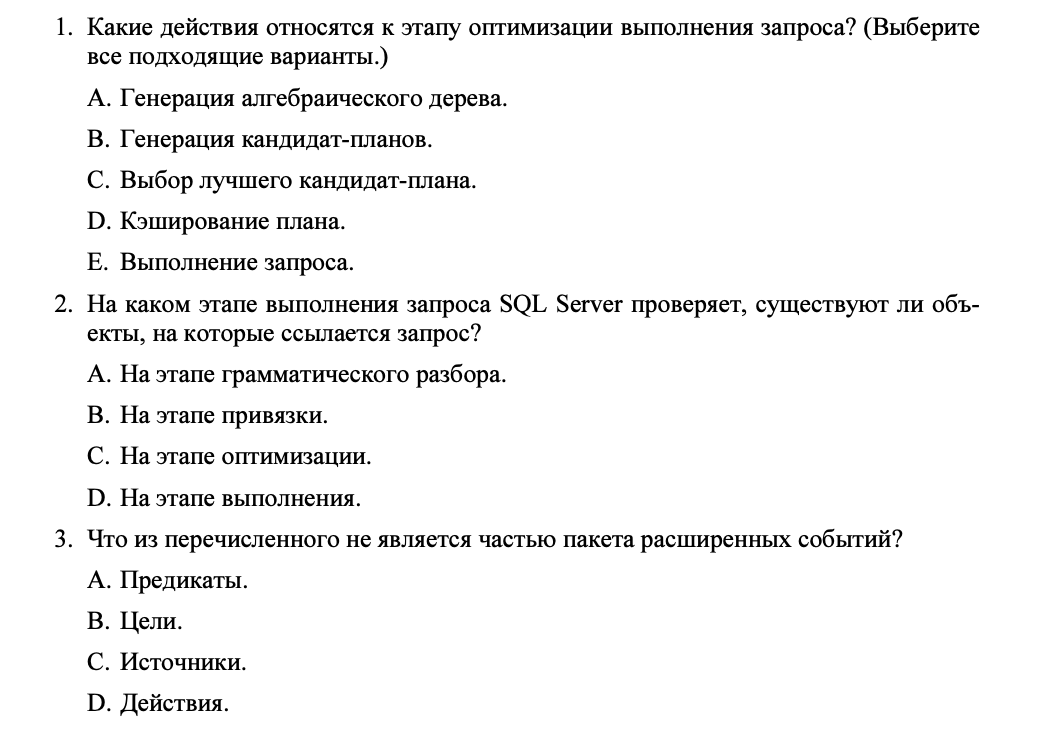
\includegraphics[width=0.7\textwidth]{img/zakrep40.png}
	\end{center}
	\captionsetup{justification=centering}
\end{figure}
\newpage

\subsection*{Ответы}

\begin{figure}[h!]
	\begin{center}
		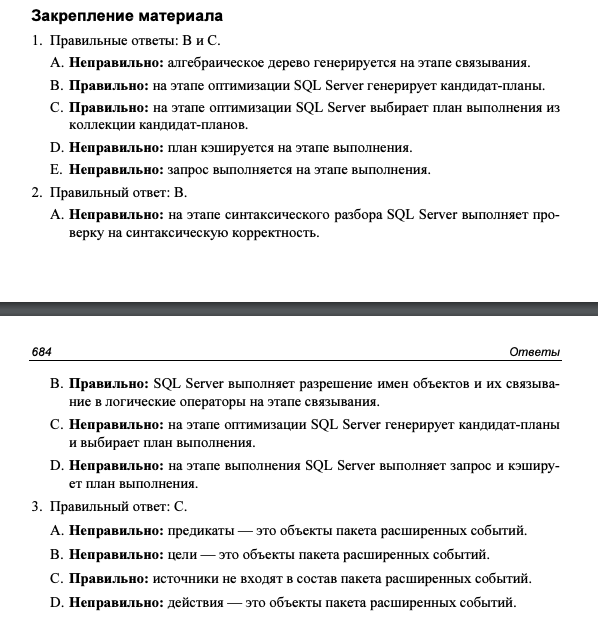
\includegraphics[width=0.6\textwidth]{img/ans40.png}
	\end{center}
	\captionsetup{justification=centering}
\end{figure}
\clearpage



\section{Использование параметров сеанса инструкции SET и анализ планов запросов}

\subsection{Параметры сеанса инструкции SET}

SQL Server хранит данные на страницах. Страница — это физическая единица на диске внутри базы данных SQL Server. Страница имеет фиксированный размер, равный 8192 байт, или 8 Кбайт. Страница принадлежит
только одному объекту, т. е. одной таблице, индексу или индексированному представлению. Далее страницы группируются в логические группы по 8 страниц, называемые экстентами. Экстент может быть смешанным, если страницы в этом
экстенте принадлежат нескольким объектам, или однородным, когда все страницы
этого экстента принадлежат только одному объекту. 



Следующий код проверяет число страниц, которые таблицы Sales.Customers и
Sales.Orders занимают в базе данных TSQL2012. 

\begin{lstlisting}[label=lst:funcReturn, language=sql]
	DBCC DROPCLEANBUFFERS;
	SET STATISTICS IO ON;
	SELECT * FROM Sales.Customers;
	SELECT * FROM Sales.Orders;
\end{lstlisting}

Обратите внимание, инструкция DBCC DROPCLEANBUFFERS удаляет данные из кэша. 

Далее приведены обозначения, используемые в возвращенной запросом информации: 

\begin{itemize}
	\item scan count (число просмотров) — количество выполненных просмотров таблицы или индекса; 
	\item logical reads (логических чтений) — количество страниц, считанных из кэша
	данных. Когда выполняется чтение целой таблицы, как в запросах из приведенного примера, это число дает оценку размера таблицы; 
	\item physical reads (физических чтений) — количество страниц, считанных с диска.
	Это число меньше, чем фактическое количество страниц, поскольку множество
	страниц находится в кэше;
	\item read-ahead reads (упреждающих чтений) — количество страниц, прочитанных
	SQL Server с упреждением; 
	\item lob logical reads (LOB логических чтений) — число страниц больших объектов
	(large object page, LOB), считанных из кэша данных. К большим объектам относятся столбцы типов VARCHAR(MAX), NVARCHAR(MAX), VARBINARY(MAX), TEXT, NTEXT,
	IMAGE, XML или большие типы данных CLR, включая системные пространственные CLR-типы GEOMETRY и GEOGRAPHY; 
	\item lob physical reads (LOB физических чтений) — число страниц типов больших
	объектов, считанных с диска; 
	\item lob read-ahead reads (LOB упреждающих чтений) — число страниц типов
	больших объектов, прочитанных SQL Server с упреждением. 
\end{itemize}


Следующая полезная для анализа производительности команда SET уровня сеанса — это команда SET STATISTICS TIME.

\begin{lstlisting}[label=lst:funcReturn, language=sql]
	SET STATISTICS TIME ON;
	DBCC DROPCLEANBUFFERS;

	SELECT C.custid, C.companyname,
 		O.orderid, O.orderdate
	FROM Sales.Customers AS C
 	INNER JOIN Sales.Orders AS O
 	ON C.custid = O.custid; 
\end{lstlisting}

\subsection{Планы выполнения}

На плане выполнения можно увидеть физические операторы, используемые в процессе выполнения.


\begin{figure}[h!]
	\begin{center}
		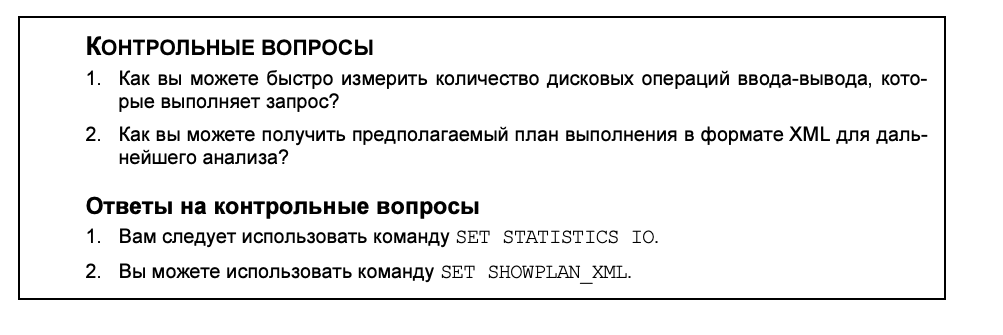
\includegraphics[width=0.9\textwidth]{img/control41.png}
	\end{center}
	\captionsetup{justification=centering}
\end{figure}

		
\subsection*{Резюме занятия}
\begin{itemize}
	\item Можно использовать параметры инструкции SET уровня сеанса для анализа
	запросов. 
	\item Можно использовать графические планы выполнения для получения подробных
	сведений о том, как SQL Server выполняет запрос. 
	\item Можно получить отображение предварительного и действительного плана выполнения. 
	\item В графическом плане выполнения можно найти подробные свойства каждого
	оператора. 
\end{itemize}


\subsection*{Закрепление материала}

\begin{figure}[h!]
	\begin{center}
		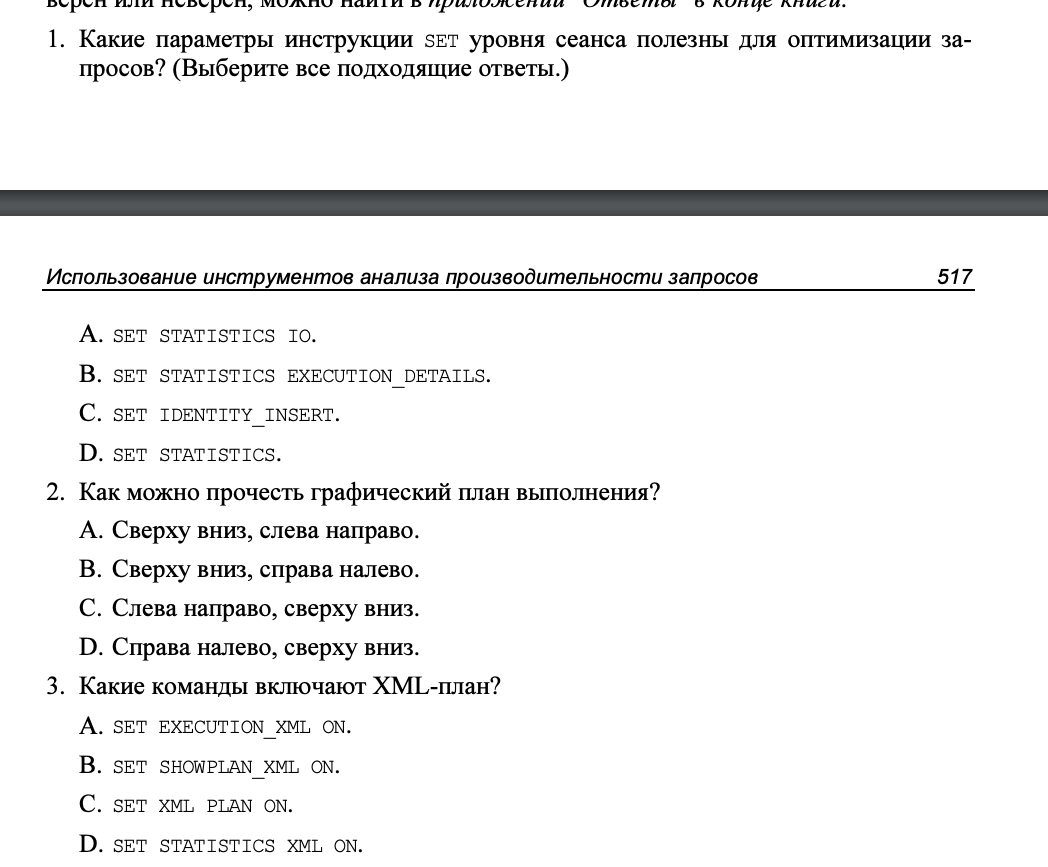
\includegraphics[width=0.9\textwidth]{img/zakrep41.png}
	\end{center}
	\captionsetup{justification=centering}
\end{figure}
\clearpage

\subsection*{Ответы}

\begin{figure}[h!]
	\begin{center}
		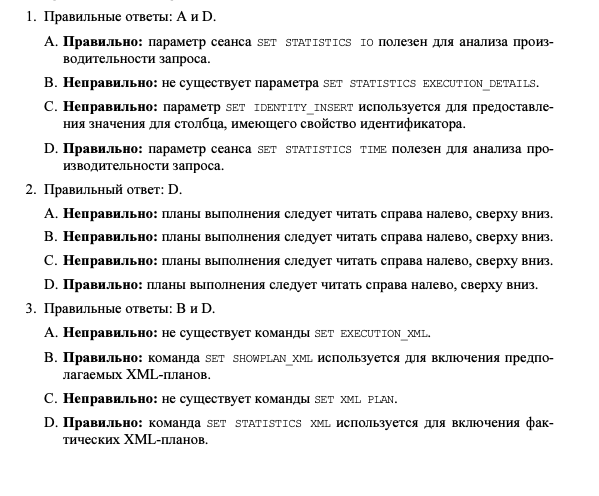
\includegraphics[width=0.9\textwidth]{img/ans41.png}
	\end{center}
	\captionsetup{justification=centering}
\end{figure}



\section{Использование динамических административных объектов}


\subsection{Введение в динамические административные объекты}

Динамические административные объекты не сохраняются ни в какой базе данных;
динамические административные объекты — это виртуальные объекты, которые
предоставляют вам доступ к собранным SQL Server данным в памяти. 

\subsection{Наиболее важные динамические административные объекты для настройки объектов}

Вы можете начать сеанс анализа со сбора системной информации. Используя относящееся к SQLOS динамическое административное представление sys dm\_os\_sys\_info, можно получить основную информацию об экземпляре сервера, как показано
в следующем запросе: 


\begin{lstlisting}[label=lst:funcReturn, language=sql]
	SELECT cpu_count AS logical_cpu_count,
	cpu_count / hyperthread_ratio AS physical_cpu_count,
	CAST(physical_memory_kb / 1024. AS int) AS physical_memory__mb,
	sqlserver_start_time
   FROM sys.dm_os_sys_info; 
\end{lstlisting}

Этот запрос возвращает информацию о количестве логических ЦП, физических
ЦП, физической памяти и времени запуска SQL Server. Последняя информация говорит о том, имеет ли смысл анализировать накопленную информацию или нет. 

Относящееся к SQLOS динамическое административное представление
sys dm\_os\_waiting\_tasks предоставляет информацию о сеансах, которые в данный
момент ожидают чего-либо.

\begin{lstlisting}[label=lst:funcReturn, language=sql]
	SELECT S.login_name, S.host_name, S.program_name,
	WT.session_id, WT.wait_duration_ms,
	WT.wait_type, WT.blocking_session_id, WT.resource_description
   FROM sys.dm_os_waiting_tasks AS WT
	INNER JOIN sys.dm_exec_sessions AS S
	ON WT.session_id = S.session_id
   WHERE s.is_user_process = 1; 
\end{lstlisting}

Связанное с выполнением запросов динамическое административное представление sys dm\_exec\_requests возвращает информацию о выполняющихся в данный момент запросах. 

\begin{lstlisting}[label=lst:funcReturn, language=sql]
	SELECT S.login_name, S.host_name, S.program_name,
	R.command, T.text,
	R.wait_type, R.wait_time, R.blocking_session_id
   FROM sys.dm_exec_requests AS R
	INNER JOIN sys.dm_exec_sessions AS S
	ON R.session_id = S.session_id
	OUTER APPLY sys.dm_exec_sql_text(R.sql_handle) AS T
   WHERE S.is_user_process = 1;
\end{lstlisting}


Вы можете извлечь множество информации о выполняемых запросах из связанного
с выполнением запросов динамического административного представления
sys dm\_exec\_query\_stats.


\subsection*{Резюме занятия}
\begin{itemize}
	\item Динамические административные объекты помогают быстро получить информацию, собранную SQL Server. 
	\item Для анализа запросов следует использовать SQLOS, относящиеся к выполнению, и связанные с индексом динамические административные объекты. 
	\item Связанные с индексом динамические административные объекты не только предоставляют полезные сведения об использовании индексов, они также информируют об отсутствующих индексах. 
\end{itemize}


\subsection*{Закрепление материала}

\begin{figure}[h!]
	\begin{center}
		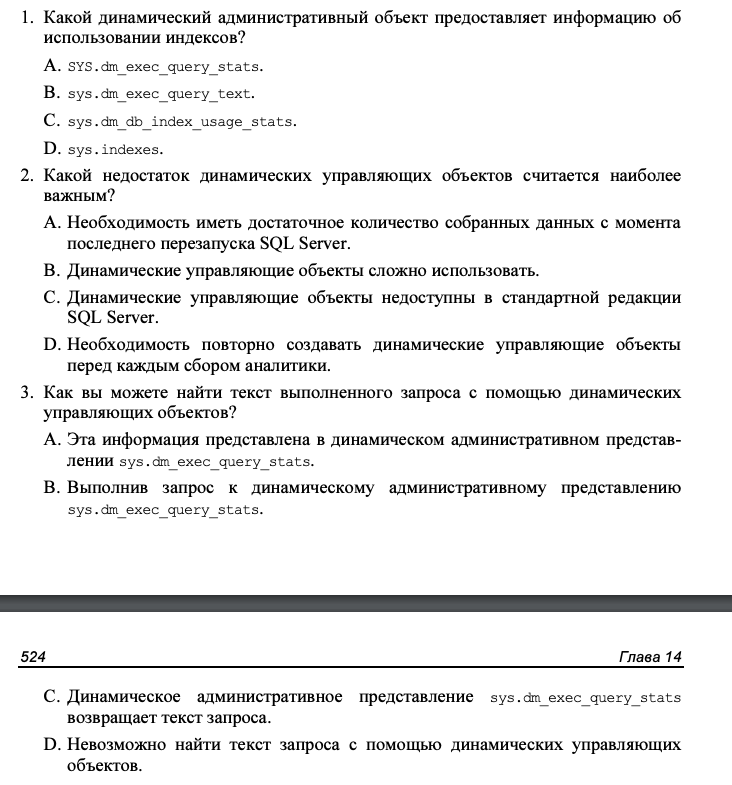
\includegraphics[width=0.7\textwidth]{img/zakrep42.png}
	\end{center}
	\captionsetup{justification=centering}
\end{figure}
\clearpage

\subsection*{Ответы}

\begin{figure}[h!]
	\begin{center}
		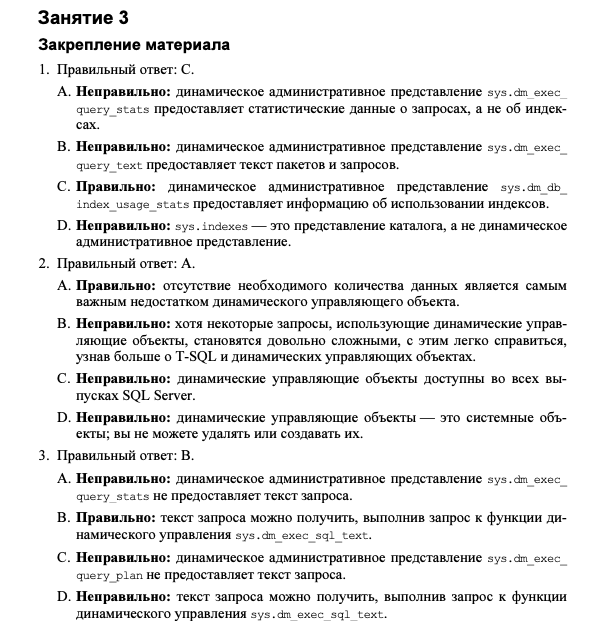
\includegraphics[width=0.9\textwidth]{img/ans42.png}
	\end{center}
	\captionsetup{justification=centering}
\end{figure}


\newpage
\subsection*{Упражнения}

\begin{figure}[h!]
	\begin{center}
		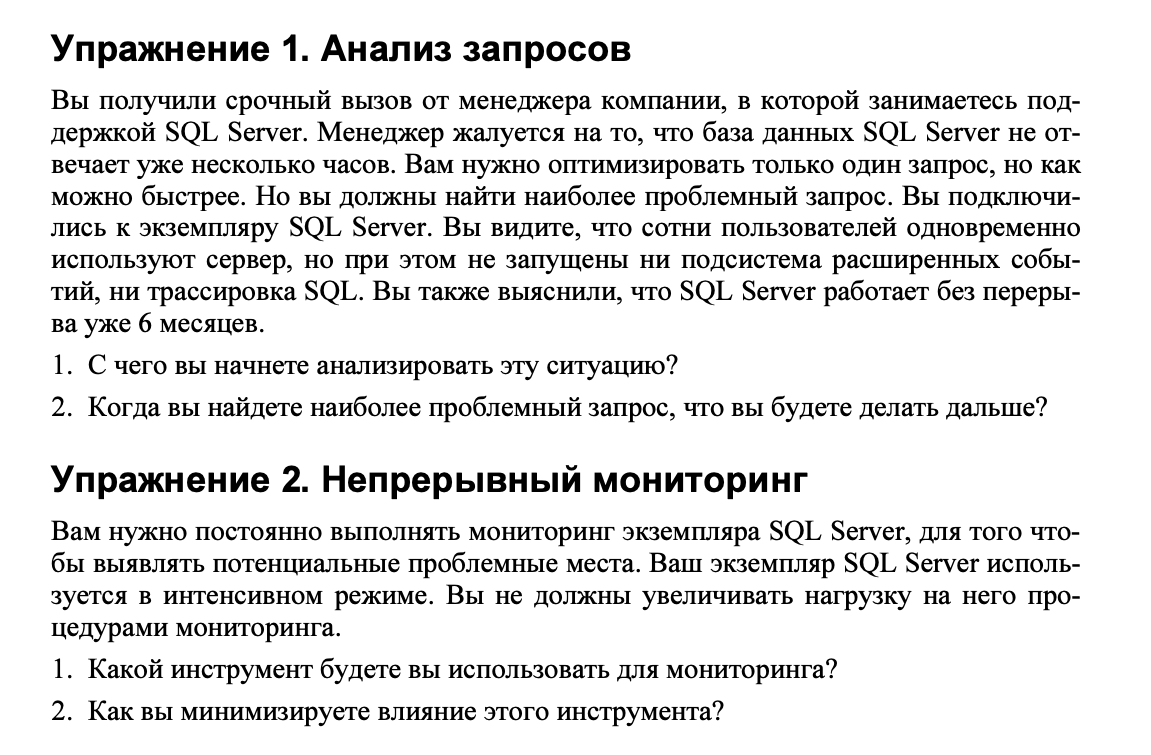
\includegraphics[width=0.9\textwidth]{img/ex18.png}
	\end{center}
	\captionsetup{justification=centering}
\end{figure}

\subsection*{Ответы}

\begin{figure}[h!]
	\begin{center}
		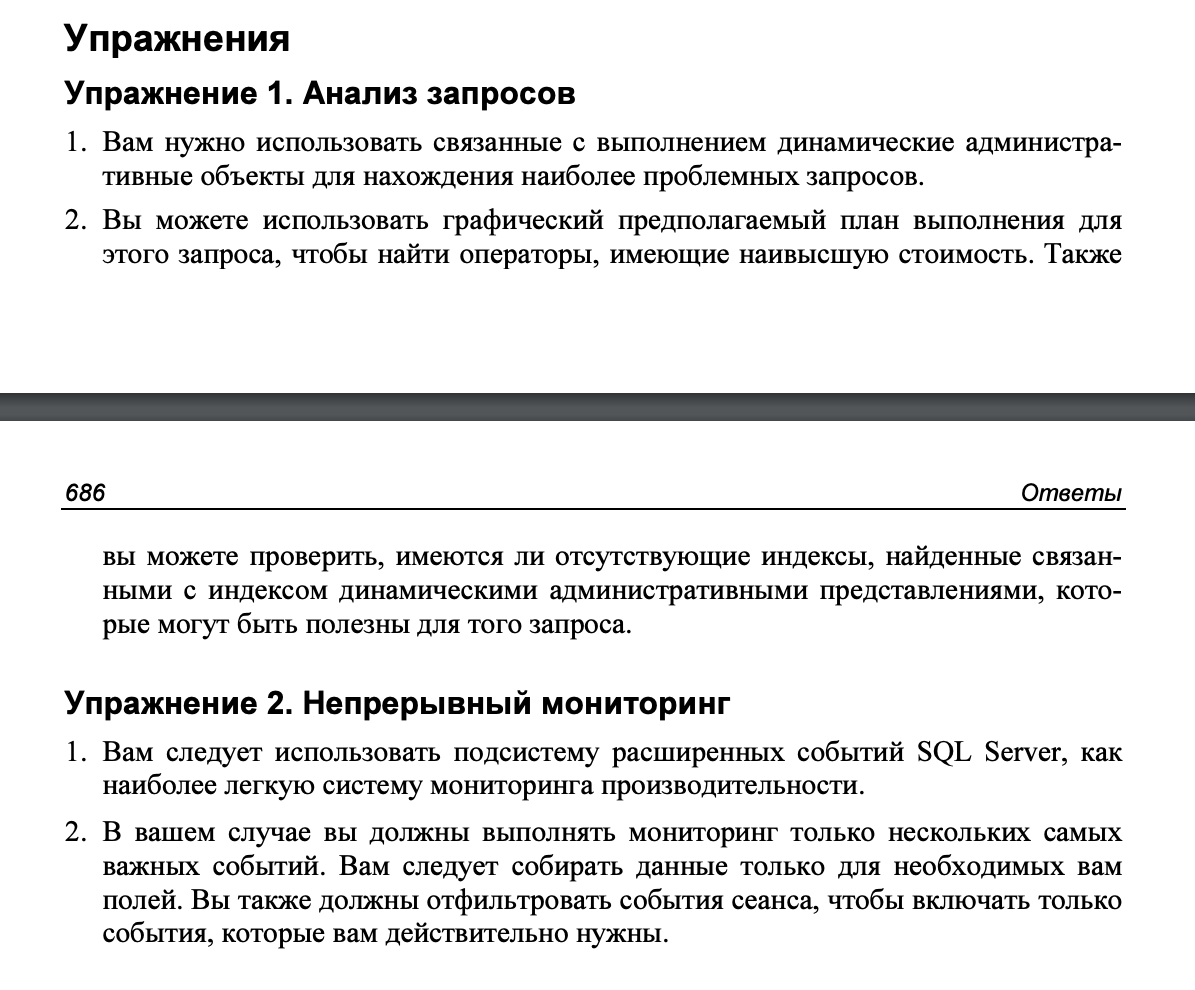
\includegraphics[width=0.9\textwidth]{img/eans18.png}
	\end{center}
	\captionsetup{justification=centering}
\end{figure}